\documentclass[12pt,a4paper]{article}

% ─── Page Layout ───────────────────────────────────────────────────────────────
\usepackage[a4paper, margin=0.8in, headheight=14pt]{geometry}

% ─── Fonts (XeLaTeX) ───────────────────────────────────────────────────────────
\usepackage{fontspec}
\usepackage{unicode-math}
\setmainfont{TeX Gyre Pagella}
\setmonofont[Scale=0.88]{TeX Gyre Cursor}
\setmathfont{Latin Modern Math}

% ─── Packages ──────────────────────────────────────────────────────────────────
\usepackage{xcolor}
\usepackage{colortbl}
\usepackage{titlesec}
\usepackage{enumitem}
\usepackage{tabularx}
\usepackage{booktabs}
\usepackage{array}
\usepackage{amsmath}
\usepackage{tikz}
\usetikzlibrary{shapes.geometric, arrows.meta, positioning, calc, fit, decorations.pathreplacing}
\usepackage{tcolorbox}
\tcbuselibrary{skins, breakable}
\usepackage{hyperref}
\usepackage{fancyhdr}
\usepackage{graphicx}
\usepackage{microtype}
\hyphenpenalty=10000
\exhyphenpenalty=10000
\sloppy
\usepackage{caption}
\usepackage{setspace}
\usepackage{multirow}
\usepackage{tocloft}

% ─── Q&A helper ────────────────────────────────────────────────────────────────
\newcommand{\Q}[1]{\textbf{#1}\par\noindent\ignorespaces}

% ─── Colour Palette ────────────────────────────────────────────────────────────
\definecolor{myred}{RGB}{196,30,58}
\definecolor{mydark}{RGB}{30,30,50}
\definecolor{mygreen}{RGB}{14,120,80}
\definecolor{myteal}{RGB}{0,130,140}
\definecolor{myamber}{RGB}{180,100,0}
\definecolor{mypurple}{RGB}{100,30,160}
\definecolor{mygray}{RGB}{246,247,249}
\definecolor{mgframe}{RGB}{180,185,200}
\definecolor{watermark}{RGB}{145,150,170}
\definecolor{hdrred}{RGB}{250,232,235}
\definecolor{hdrgreen}{RGB}{220,244,233}
\definecolor{hdrteal}{RGB}{220,242,244}
\definecolor{hdramber}{RGB}{253,242,215}
\definecolor{hdrpurple}{RGB}{238,228,255}
\definecolor{hdrgray}{RGB}{238,240,245}
\definecolor{rowalt}{RGB}{250,251,253}

% ─── Section Formatting ────────────────────────────────────────────────────────
\titleformat{\section}
  {\large\bfseries\color{myred}}{\thesection.}{0.5em}{}
  [\vspace{1pt}{\color{myred}\rule{\linewidth}{0.8pt}}]
\titleformat{\subsection}
  {\normalsize\bfseries\color{myteal}}{\thesubsection}{0.5em}{}
\titlespacing*{\section}{0pt}{18pt}{7pt}
\titlespacing*{\subsection}{0pt}{11pt}{4pt}

% ─── Paragraph ─────────────────────────────────────────────────────────────────
\setlength{\parindent}{0pt}
\setlength{\parskip}{4pt}

% ─── TOC Styling ───────────────────────────────────────────────────────────────
\renewcommand{\cfttoctitlefont}{\large\bfseries\color{myred}}
\renewcommand{\cftaftertoctitle}{\par\noindent{\color{myred}\rule{\linewidth}{0.8pt}}}
\setlength{\cftbeforetoctitleskip}{0pt}
\setlength{\cftaftertoctitleskip}{6pt}
\renewcommand{\cftsecfont}{\normalsize\bfseries\color{mydark}}
\renewcommand{\cftsecpagefont}{\normalsize\bfseries\color{mydark}}
\renewcommand{\cftsecleader}{\cftdotfill{\cftdotsep}}
\setlength{\cftbeforesecskip}{7pt}
\renewcommand{\cftsubsecfont}{\small\color{mydark}}
\renewcommand{\cftsubsecpagefont}{\small\color{mydark}}
\setlength{\cftbeforesubsecskip}{3pt}
\setlength{\cftsubsecindent}{1.4em}

% ─── Table helpers ─────────────────────────────────────────────────────────────
\renewcommand{\arraystretch}{1.45}
\setlength{\tabcolsep}{6pt}
\arrayrulecolor{mydark}
\newcolumntype{B}[1]{>{\small\bfseries\raggedright\arraybackslash}m{#1}}
\newcolumntype{Y}{>{\small\raggedright\arraybackslash}X}
\renewcommand{\tabularxcolumn}[1]{m{#1}}

% ─── Header / Footer ───────────────────────────────────────────────────────────
\pagestyle{fancy}
\fancyhf{}
\fancyhead[L]{\small\color{myred}\textbf{PE-EC801A}\;\color{mydark}--- Antennas and Propagation}
\fancyhead[R]{\small\color{myteal}\textbf{Module 2 Notes}}
\fancyfoot[C]{\small\color{mydark}\thepage}
\fancyfoot[R]{\small\color{watermark}\textit{\copyright\ Biraj}}
\renewcommand{\headrulewidth}{0.5pt}
\renewcommand{\footrulewidth}{0.3pt}

% ─── Hyperref ──────────────────────────────────────────────────────────────────
\hypersetup{
  colorlinks=true, linkcolor=myteal, urlcolor=myteal,
  pdfauthor={Biraj Sarkar},
  pdftitle={PE-EC801A --- Module 2 Notes}
}

% ─── tcolorbox styles ──────────────────────────────────────────────────────────
\tcbset{
  tikzbox/.style={
    colback=mygray, colframe=mgframe, boxrule=0.6pt, arc=4pt,
    left=8pt, right=8pt, top=6pt, bottom=6pt,
    colbacktitle=mgframe, coltitle=mydark,
    fonttitle=\small\bfseries
  },
  defbox/.style={
    colback=hdrgreen, colframe=mygreen, boxrule=0.8pt, arc=4pt,
    left=9pt, right=9pt, top=6pt, bottom=6pt,
    colbacktitle=mygreen, coltitle=white,
    fonttitle=\small\bfseries
  },
  formulabox/.style={
    colback=hdrteal, colframe=myteal, boxrule=0.8pt, arc=4pt,
    left=9pt, right=9pt, top=7pt, bottom=7pt,
    colbacktitle=myteal, coltitle=white,
    fonttitle=\small\bfseries
  },
  examplebox/.style={
    colback=hdramber, colframe=myamber, boxrule=0.8pt, arc=4pt,
    left=9pt, right=9pt, top=6pt, bottom=6pt,
    colbacktitle=myamber, coltitle=white,
    fonttitle=\small\bfseries
  },
  masonbox/.style={
    colback=hdrpurple, colframe=mypurple, boxrule=0.8pt, arc=4pt,
    left=9pt, right=9pt, top=6pt, bottom=6pt,
    colbacktitle=mypurple, coltitle=white,
    fonttitle=\small\bfseries
  },
  exambox/.style={
    colback=hdrpurple, colframe=mypurple, boxrule=1pt, arc=5pt,
    left=10pt, right=10pt, top=8pt, bottom=8pt,
    colbacktitle=mypurple, coltitle=white,
    fonttitle=\bfseries,
    breakable, title after break={\textbf{Frequently Asked / Viva Questions (contd.)}}}
}
\tcbset{breakable}

% ─── TikZ styles ───────────────────────────────────────────────────────────────
\tikzset{
  block/.style={rectangle, draw=myteal, fill=hdrteal,
    text width=2.4cm, align=center, minimum height=0.95cm,
    font=\small, rounded corners=3pt, line width=0.7pt},
  redblock/.style={rectangle, draw=myred, fill=hdrred,
    text width=2.4cm, align=center, minimum height=0.95cm,
    font=\small, rounded corners=3pt, line width=0.7pt},
  netnode/.style={rectangle, draw=myteal, fill=hdrteal,
    text width=1.5cm, align=center, minimum height=0.8cm,
    font=\small, rounded corners=3pt, line width=0.7pt},
  sumjunc/.style={circle, draw=myamber, fill=hdramber,
    minimum size=0.62cm, font=\small, line width=0.8pt},
  snode/.style={circle, draw=mypurple, fill=hdrpurple,
    minimum size=0.55cm, font=\footnotesize, line width=0.7pt},
  arrow/.style={-Stealth, thick, color=mydark},
  redarrow/.style={-Stealth, thick, color=myred},
  line/.style={thick, color=mydark}
}

% ═══════════════════════════════════════════════════════════════════════════════
\begin{document}
% ═══════════════════════════════════════════════════════════════════════════════

\begin{center}
  {\LARGE\bfseries\color{myred} PE-EC801A --- Antennas and Propagation}\\[5pt]
  {\normalsize\color{mydark} Semester VIII \quad$\bullet$\quad 3L:0T:0P \quad$\bullet$\quad 3 Credits}\\[3pt]
  {\normalsize\color{myteal}\textbf{Module 2 Exam Notes}}\\[3pt]
  {\small\color{mydark} CGEC \;$|$\; B.Tech ECE (2023--27) \;$|$\; \textit{Biraj Sarkar}}
\end{center}
\vspace{2pt}
\noindent{\color{myred}\rule{\linewidth}{1.5pt}}
\vspace{2pt}

\hypersetup{linkcolor=mydark}
\tableofcontents
\hypersetup{linkcolor=myteal}
\newpage

% ===============================================================================
\section{Infinitesimal Dipole}
% ===============================================================================

\begin{tcolorbox}[defbox, title={\textbf{Definition of Infinitesimal Dipole}}]
An \textbf{infinitesimal dipole} (also known as a Hertzian dipole) is a thin linear antenna whose length $dl$ is extremely small compared to the wavelength ($dl \ll \lambda$) and whose current is assumed to be uniform ($I(z) = I_0 = \text{constant}$) over its entire length.
\end{tcolorbox}

\subsection{Coordinate System and Potential Derivation}
Consider a wire of length $dl$ placed symmetrically at the origin along the $z$-axis. Since the current is along $z$, the current density is $\vec{J} = \hat{a}_z I_0 \delta(x')\delta(y')$ for $-dl/2 \le z' \le dl/2$. 

\begin{tcolorbox}[tikzbox, title={Infinitesimal Dipole Geometry}]
\centering
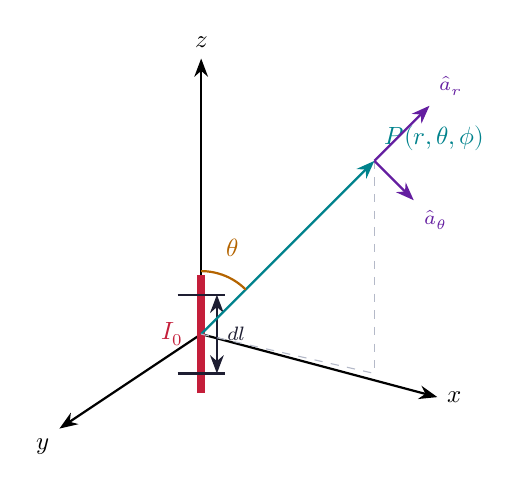
\begin{tikzpicture}[scale=1.0]
  % Spherical coordinates axes
  \draw[-Stealth, thick] (0,0) -- (0,3.5) node[above, font=\small] {$z$};
  \draw[-Stealth, thick] (0,0) -- (3.0,-0.8) node[right, font=\small] {$x$};
  \draw[-Stealth, thick] (0,0) -- (-1.8,-1.2) node[below left, font=\small] {$y$};

  % Dipole wire
  \draw[line width=3pt, color=myred] (0,-0.75) -- (0,0.75);
  \draw[thick, color=mydark] (-0.3, 0.5) -- (0.3, 0.5);
  \draw[thick, color=mydark] (-0.3, -0.5) -- (0.3, -0.5);
  \draw[Stealth-Stealth, thick, color=mydark] (0.2, -0.5) -- (0.2, 0.5) node[midway, right, font=\scriptsize] {$dl$};
  \node[left=3pt, font=\small\bfseries\color{myred}] at (0,0) {$I_0$};

  % Vector to observation point
  \draw[-Stealth, thick, color=myteal] (0,0) -- (2.2,2.2) node[above right, font=\small] {$P(r, \theta, \phi)$};
  \draw[dashed, color=mgframe] (2.2,2.2) -- (2.2,-0.5);
  \draw[dashed, color=mgframe] (0,0) -- (2.2,-0.5);

  % Angles
  \draw[thick, color=myamber] (0,0.8) arc (90:45:0.8);
  \node[color=myamber, font=\small\bfseries] at (0.4, 1.1) {$\theta$};

  % Unit vectors
  \draw[-Stealth, thick, color=mypurple] (2.2,2.2) -- (2.9,2.9) node[above right, font=\scriptsize] {$\hat{a}_r$};
  \draw[-Stealth, thick, color=mypurple] (2.2,2.2) -- (2.7,1.7) node[below right, font=\scriptsize] {$\hat{a}_\theta$};

\end{tikzpicture}
\end{tcolorbox}

The magnetic vector potential $\vec{A}$ at a distance $r$ (since $r \gg dl$) is:
\[
\vec{A}(r) = \hat{a}_z \frac{\mu I_0 dl}{4\pi r} e^{-jkr}
\]
Using coordinate transformations, the spherical components of $\vec{A}$ are:
\[
A_r = A_z \cos\theta = \frac{\mu I_0 dl \cos\theta}{4\pi r} e^{-jkr}
\]
\[
A_\theta = -A_z \sin\theta = -\frac{\mu I_0 dl \sin\theta}{4\pi r} e^{-jkr}
\]
\[
A_\phi = 0
\]

\subsection{Electromagnetic Field Equations}
By applying Maxwell's relations ($\vec{H} = \frac{1}{\mu} \nabla \times \vec{A}$ and $\vec{E} = \frac{1}{j\omega\epsilon} \nabla \times \vec{H}$), we obtain the complete field equations:
\[
H_\phi = j \frac{k I_0 dl \sin\theta}{4\pi r} \left[ 1 + \frac{1}{jkr} \right] e^{-jkr}
\]
\[
E_r = \frac{2 I_0 dl \eta \cos\theta}{4\pi r^2} \left[ 1 + \frac{1}{jkr} \right] e^{-jkr}
\]
\[
E_\theta = j \frac{k I_0 dl \eta \sin\theta}{4\pi r} \left[ 1 + \frac{1}{jkr} - \frac{1}{(kr)^2} \right] e^{-jkr}
\]
where $\eta = \sqrt{\mu/\epsilon} \approx 120\pi \approx 377\,\Omega$ is the intrinsic impedance of free space. Other components $H_r = H_\theta = E_\phi = 0$.

\subsection{Far-Field Approximation and Radiation Resistance}
For the far field ($kr \gg 1$), terms containing $1/(kr)^2$ and $1/(kr)^3$ can be neglected. The fields simplify to:
\[
H_\phi \approx j \frac{I_0 k dl \sin\theta}{4\pi r} e^{-jkr}
\]
\[
E_\theta \approx j \eta \frac{I_0 k dl \sin\theta}{4\pi r} e^{-jkr}
\]
The total power radiated is found by integrating the Poynting vector over a closed sphere:
\[
P_{rad} = \int_{0}^{2\pi}\int_{0}^{\pi} \frac{1}{2} \text{Re}(E_\theta H_\phi^*) r^2 \sin\theta \, d\theta \, d\phi = 40 \pi^2 I_0^2 \left(\frac{dl}{\lambda}\right)^{\!2}
\]
Since $P_{rad} = \frac{1}{2} I_0^2 R_r$, the radiation resistance $R_r$ of an infinitesimal dipole is:
\[
R_r = 80 \pi^2 \left(\frac{dl}{\lambda}\right)^{\!2}
\]

\begin{tcolorbox}[defbox, title={\textbf{Note: The Short Dipole}}]
For a \textbf{short dipole} (length $l \ll \lambda$, but current decreases linearly from $I_0$ at the center to $0$ at the ends), the average current is $I_0/2$. The radiation resistance is $1/4$ of the infinitesimal dipole:
\[
R_r = 20\pi^2 \left(\frac{l}{\lambda}\right)^{\!2}
\]
\end{tcolorbox}

% ===============================================================================
\section{Finite-Length Dipole}
% ===============================================================================

When the antenna length is comparable to the wavelength, the current is no longer uniform. It forms a standing wave with a sinusoidal distribution (assuming thin wire and zero current at the ends).

\subsection{Current Distribution}
For a dipole of length $l$ placed along the $z$-axis, the current distribution is:
\[
I(z') = I_0 \sin\left[ k \left( \frac{l}{2} - |z'| \right) \right], \quad -l/2 \le z' \le l/2
\]

\begin{tcolorbox}[tikzbox, title={Current Distributions on Dipoles}]
\centering
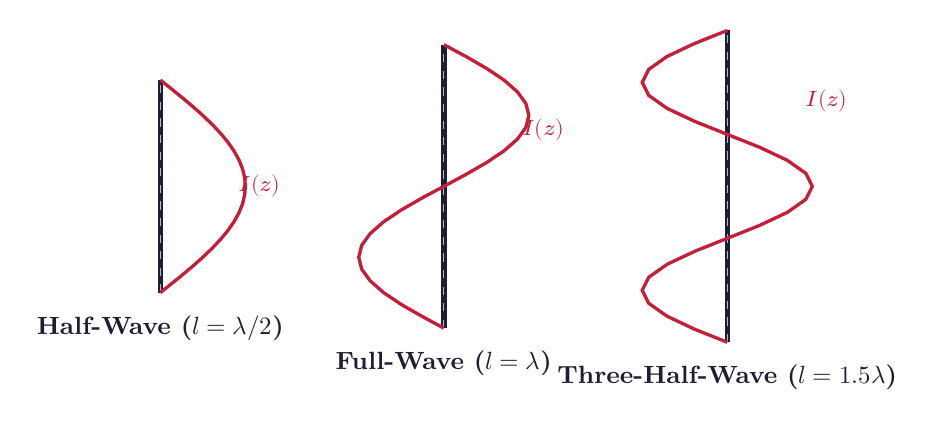
\begin{tikzpicture}[scale=0.9]
  % 1/2 Wave Dipole
  \begin{scope}[xshift=-4cm]
    \draw[line width=2pt, color=mydark] (0,-1.5) -- (0,1.5);
    \draw[dashed, color=mgframe] (0,-1.5) -- (0,1.5);
    % Current curve
    \draw[very thick, color=myred, domain=-1.5:1.5] plot ({1.2*cos(90*\x/1.5)}, \x);
    \node[font=\footnotesize\bfseries\color{myred}] at (1.4,0) {$I(z)$};
    \node[font=\small\bfseries\color{mydark}] at (0,-2.0) {Half-Wave ($l = \lambda/2$)};
  \end{scope}

  % Full Wave Dipole
  \begin{scope}[xshift=0cm]
    \draw[line width=2pt, color=mydark] (0,-2.0) -- (0,2.0);
    \draw[dashed, color=mgframe] (0,-2.0) -- (0,2.0);
    % Current curve
    \draw[very thick, color=myred, domain=-2:2] plot ({1.2*sin(180*\x/2.0)}, \x);
    \node[font=\footnotesize\bfseries\color{myred}] at (1.4,0.8) {$I(z)$};
    \node[font=\small\bfseries\color{mydark}] at (0,-2.5) {Full-Wave ($l = \lambda$)};
  \end{scope}

  % 3/2 Wave Dipole
  \begin{scope}[xshift=4cm]
    \draw[line width=2pt, color=mydark] (0,-2.2) -- (0,2.2);
    \draw[dashed, color=mgframe] (0,-2.2) -- (0,2.2);
    % Current curve
    \draw[very thick, color=myred, domain=-2.2:2.2] plot ({1.2*cos(270*\x/2.2)}, \x);
    \node[font=\footnotesize\bfseries\color{myred}] at (1.4,1.2) {$I(z)$};
    \node[font=\small\bfseries\color{mydark}] at (0,-2.7) {Three-Half-Wave ($l = 1.5\lambda$)};
  \end{scope}
\end{tikzpicture}
\end{tcolorbox}

\subsection{Far-Field Radiation Pattern}
By treating the finite dipole as an infinite sum of infinitesimal dipoles and integrating the contributions, the far-field electric field is:
\[
E_\theta \approx j \eta \frac{I_0 e^{-jkr}}{2\pi r} \left[ \frac{\cos\left(\frac{kl}{2}\cos\theta\right) - \cos\left(\frac{kl}{2}\right)}{\sin\theta} \right]
\]
\[
H_\phi = \frac{E_\theta}{\eta}
\]

\subsection{The Half-Wave Dipole (\texorpdfstring{$l = \lambda/2$}{l = lambda/2})}
Setting $l = \lambda/2$ (and thus $kl/2 = \pi/2$) in the field equations:
\[
E_\theta \approx j \eta \frac{I_0 e^{-jkr}}{2\pi r} \left[ \frac{\cos\left(\frac{\pi}{2}\cos\theta\right)}{\sin\theta} \right]
\]
\begin{itemize}[leftmargin=*, itemsep=3pt]
  \item \textbf{Radiation Resistance:} $R_r \approx 73\,\Omega$.
  \item \textbf{Input Impedance:} $Z_{in} \approx 73 + j 42.5\,\Omega$ (inductive reactant due to end effects).
  \item \textbf{Resonant Length:} To make the input impedance purely real ($Z_{in} \approx 73 + j0\,\Omega$), the dipole is shortened slightly by about $5\%$ ($l \approx 0.47\lambda$–$0.48\lambda$).
  \item \textbf{Directivity ($D_0$):} $1.64$ ($2.15\,\text{dBi}$).
  \item \textbf{HPBW:} $78^\circ$.
\end{itemize}

% ===============================================================================
\section{Linear Elements Near Conductors (Image Theory)}
% ===============================================================================

To analyze antennas placed near flat, perfectly conducting ground planes, we replace the ground plane with an equivalent virtual antenna below the plane. This is called \textbf{Image Theory}.

\begin{tcolorbox}[tikzbox, title={Image Theory Equivalents}]
\centering
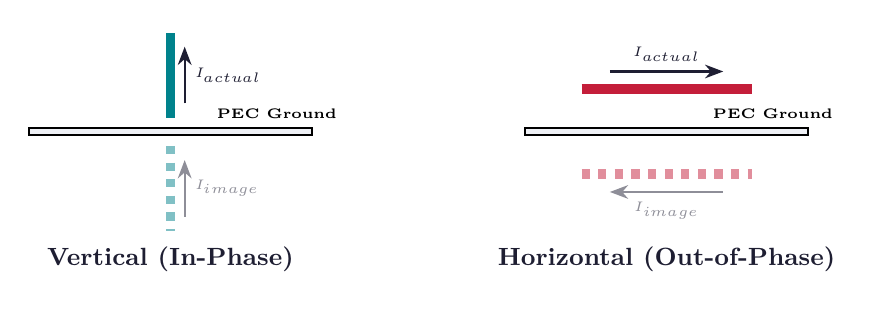
\begin{tikzpicture}[scale=0.9]
  % Vertical antenna case
  \begin{scope}[xshift=-3.5cm]
    \draw[thick, fill=hdrgray] (-2,-0.05) rectangle (2,0.05);
    \node[above, font=\tiny\bfseries] at (1.5,0.05) {PEC Ground};
    
    % Actual dipole
    \draw[line width=3.5pt, color=myteal] (0,0.2) -- (0,1.4);
    \draw[-Stealth, thick, color=mydark] (0.2,0.4) -- (0.2,1.2) node[midway, right, font=\tiny] {$I_{actual}$};
    
    % Image dipole
    \draw[line width=3.5pt, color=myteal!50, dashed] (0,-0.2) -- (0,-1.4);
    \draw[-Stealth, thick, color=mydark!50] (0.2,-1.2) -- (0.2,-0.4) node[midway, right, font=\tiny] {$I_{image}$};
    \node[font=\small\bfseries\color{mydark}] at (0,-1.8) {Vertical (In-Phase)};
  \end{scope}

  % Horizontal antenna case
  \begin{scope}[xshift=3.5cm]
    \draw[thick, fill=hdrgray] (-2,-0.05) rectangle (2,0.05);
    \node[above, font=\tiny\bfseries] at (1.5,0.05) {PEC Ground};
    
    % Actual dipole
    \draw[line width=3.5pt, color=myred] (-1.2,0.6) -- (1.2,0.6);
    \draw[-Stealth, thick, color=mydark] (-0.8,0.85) -- (0.8,0.85) node[midway, above, font=\tiny] {$I_{actual}$};
    
    % Image dipole
    \draw[line width=3.5pt, color=myred!50, dashed] (-1.2,-0.6) -- (1.2,-0.6);
    \draw[Stealth-, thick, color=mydark!50] (-0.8,-0.85) -- (0.8,-0.85) node[midway, below, font=\tiny] {$I_{image}$};
    \node[font=\small\bfseries\color{mydark}] at (0,-1.8) {Horizontal (Out-of-Phase)};
  \end{scope}
\end{tikzpicture}
\end{tcolorbox}

\subsection{Boundary Rules for Image Currents}
\begin{itemize}[leftmargin=*, itemsep=3pt]
  \item \textbf{Vertical Element:} A vertical current element at distance $h$ above a ground plane has an image element of the same length and direction (in-phase) at distance $h$ below the plane.
  \item \textbf{Horizontal Element:} A horizontal current element at distance $h$ above a ground plane has an image element of the same length but opposite direction (out-of-phase) at distance $h$ below the plane.
\end{itemize}

% ===============================================================================
\section{Dipoles for Mobile Communication (Monopoles)}
% ===============================================================================

For mobile handsets and base stations, it is often impractical to use a symmetric double-sided dipole. Instead, a \textbf{monopole antenna} (a single wire placed perpendicular to a conducting ground plane) is used.

\subsection{The Quarter-Wave Monopole (\texorpdfstring{$l = \lambda/4$}{l = lambda/4})}
Using image theory, a monopole of length $l = \lambda/4$ on a perfect ground plane is equivalent to a half-wave dipole ($l = \lambda/2$) in free space, but only for the upper half-space ($z \ge 0$).

\begin{itemize}[leftmargin=*, itemsep=3pt]
  \item \textbf{Fields ($z \ge 0$):} Identical to half-wave dipole fields.
  \item \textbf{Fields ($z < 0$):} Zero (shielded by ground plane).
  \item \textbf{Radiated Power ($P_{rad, mono}$):} Since it radiates only into the upper hemisphere, the radiated power for the same input current is half that of a dipole:
  \[
  P_{rad, monopole} = \frac{1}{2} P_{rad, dipole}
  \]
  \item \textbf{Radiation Resistance ($R_{r, mono}$):}
  \[
  R_{r, monopole} = \frac{1}{2} R_{r, dipole} = \frac{73}{2} \approx 36.5\,\Omega
  \]
  \item \textbf{Directivity ($D_{mono}$):} Since the power is focused into half the volume, the directivity is double that of a dipole:
  \[
  D_{monopole} = 2 \times D_{dipole} = 2 \times 1.64 = 3.28 \quad (5.16\,\text{dBi})
  \]
\end{itemize}

% ===============================================================================
\section{Small Circular Loop Antenna}
% ===============================================================================

\begin{tcolorbox}[defbox, title={\textbf{Definition of Small Circular Loop}}]
A \textbf{small circular loop antenna} is a loop antenna of radius $a$ whose circumference is much smaller than the wavelength ($2\pi a \ll \lambda$), resulting in a uniform current distribution $I(z) = I_0$ along the loop.
\end{tcolorbox}

\subsection{Far-Field Radiated Fields}
By using the magnetic vector potential $\vec{A} = \hat{a}_\phi A_\phi$, the far fields for a loop with area $S = \pi a^2$ are:
\[
E_\phi \approx \frac{\eta k^2 I_0 S \sin\theta}{4\pi r} e^{-jkr}
\]
\[
H_\theta \approx -\frac{E_\phi}{\eta} \approx -\frac{k^2 I_0 S \sin\theta}{4\pi r} e^{-jkr}
\]

\subsection{Radiation Resistance}
The power radiated by the loop is integrated, leading to the radiation resistance:
\[
R_r = 31200 \left( \frac{S}{\lambda^2} \right)^{\!2} = 31200 \left( \frac{\pi a^2}{\lambda^2} \right)^{\!2} \approx 320\pi^4 \left( \frac{a}{\lambda} \right)^{\!4}
\]

\begin{tcolorbox}[defbox, title={\textbf{Important Note: Small Loop as a Magnetic Dipole}}]
The radiation pattern of a small loop has a torus/donut shape ($f(\theta) = \sin\theta$), which is identical to the pattern of an infinitesimal electric dipole. Thus, a small loop behaves as a \textbf{magnetic dipole} perpendicular to the plane of the loop. However, its radiation resistance is much smaller than that of an electric dipole of similar size, making it a less efficient radiator (often used primarily for receiving, e.g., AM radio).
\end{tcolorbox}

% ===============================================================================
% MANDATORY QUICK REVISION PAGE
% ===============================================================================
\newpage
\begin{center}
  {\large\bfseries\color{myred} Quick Revision --- Module 2}\\[3pt]
  {\small\color{mydark} Wire and Loop Antennas $|$ PE-EC801A}
\end{center}
\noindent{\color{myred}\rule{\linewidth}{1.2pt}}
\vspace{4pt}

\begin{tcolorbox}[formulabox, title={\textbf{Key Formulas and Metrics at a Glance}}]
\renewcommand{\arraystretch}{1.35}
\begin{tabularx}{\linewidth}{B{5.2cm} X}
Infinitesimal Dipole $R_r$ & $R_r = 80\pi^2 \left(\frac{dl}{\lambda}\right)^2$ \quad ($dl \ll \lambda$, uniform current) \\[4pt]
Short Dipole $R_r$ & $R_r = 20\pi^2 \left(\frac{l}{\lambda}\right)^2$ \quad ($l \ll \lambda$, linear current) \\[4pt]
Half-Wave Dipole $R_r$ \& $D_0$ & $R_r \approx 73\,\Omega$, \quad $D_0 \approx 1.64$ ($2.15\,\text{dBi}$) \\[4pt]
Quarter-Wave Monopole $R_r$ \& $D_0$ & $R_r \approx 36.5\,\Omega$, \quad $D_0 \approx 3.28$ ($5.16\,\text{dBi}$) \\[4pt]
Small Loop $R_r$ & $R_r \approx 31200 \left(\frac{S}{\lambda^2}\right)^2$ \quad ($S = \pi a^2$) \\[4pt]
Dipole Current Profile & $I(z) = I_0 \sin\left[k(l/2 - |z|)\right]$ \\[4pt]
Resonant Dipole Length & $l_{resonant} \approx 0.47\lambda$–$0.48\lambda$ \quad (removes $+j42.5\,\Omega$ reactance) \\
\end{tabularx}
\end{tcolorbox}

\begin{tcolorbox}[defbox, title={\textbf{One-Line Definitions}}]
\begin{itemize}[leftmargin=*, itemsep=2pt, topsep=0pt]
  \item \textbf{Hertzian Dipole:} A theoretical, infinitely thin dipole antenna of length much smaller than a wavelength, carrying uniform current.
  \item \textbf{Resonant Antenna:} An antenna whose input impedance is purely resistive ($X_{in} = 0$) at its operating frequency.
  \item \textbf{Image Theory:} A mathematical method replacing a conducting boundary with virtual mirror-image current sources.
  \item \textbf{Quarter-Wave Monopole:} A single vertical wire of length $\lambda/4$ placed above a conducting ground plane.
  \item \textbf{Magnetic Dipole:} The dual of an electric dipole; represented physically by a small circular loop antenna.
\end{itemize}
\end{tcolorbox}

\begin{tcolorbox}[exambox, title={\textbf{Frequently Asked / Viva Questions}}]
\begin{enumerate}[topsep=0pt, label=\textbf{Q\arabic*.}, itemsep=5pt]
  \item \Q{What is the difference between an infinitesimal dipole and a short dipole?}
    An infinitesimal dipole has a constant, uniform current along its length ($dl \ll \lambda$). A short dipole has current that drops off linearly from the center to zero at the ends ($l \ll \lambda$). Because of this current profile, the radiation resistance of a short dipole is one-quarter of that of an infinitesimal dipole.
  \item \Q{Why does a half-wave dipole require shortening for resonance?}
    A physical half-wave dipole ($l = 0.5\lambda$) has an input impedance of $Z_{in} \approx 73 + j42.5\,\Omega$. To eliminate the inductive reactance and make it resonant ($X_{in} = 0$), the antenna is shortened slightly to about $0.47\lambda$–$0.48\lambda$.
  \item \Q{Compare a half-wave dipole and a quarter-wave monopole antenna.}
    A quarter-wave monopole on a ground plane has half the radiation resistance ($36.5\,\Omega$ vs. $73\,\Omega$) and twice the directivity ($3.28$ vs. $1.64$, or $5.16\,\text{dBi}$ vs. $2.15\,\text{dBi}$) of a free-space half-wave dipole, because its radiation is restricted to the upper hemisphere.
  \item \Q{Explain how the image of a horizontal dipole differs from a vertical dipole.}
    For a vertical dipole, the image current is in the same direction (in-phase). For a horizontal dipole, the image current is in the opposite direction (out-of-phase), which causes the radiated field to cancel at grazing angles ($0^\circ$ elevation).
  \item \Q{Why are small loop antennas rarely used as transmitting antennas?}
    Small loop antennas have a very small radiation resistance (proportional to $(a/\lambda)^4$). This makes their radiation efficiency extremely low, as most input power is lost as heat in the conductor. They are, however, excellent for receiving applications (like AM radio) where noise levels are high and matching can be tuned.
  \item \Q{Write the far-field expressions for a half-wave dipole.}
    $E_\theta = j 120 I_0 \frac{e^{-jkr}}{2 r} \left[ \frac{\cos\left(\frac{\pi}{2}\cos\theta\right)}{\sin\theta} \right]$ and $H_\phi = \frac{E_\theta}{\eta}$. Other field components are zero.
  \item \Q{What is the input impedance of a practical half-wave dipole at resonance?}
    At resonance, the input reactance is tuned to zero, and the input impedance is purely resistive: $Z_{in} \approx 73\,\Omega$.
\end{enumerate}
\end{tcolorbox}

\begin{tcolorbox}[tikzbox, title={Comparison of Wire and Loop Antennas}]
\centering
\renewcommand{\arraystretch}{1.55}
{\renewcommand{\arraystretch}{1.55}%
\begin{tabularx}{\linewidth}{|B{3.2cm}|Y|Y|Y|}
\hline
\multicolumn{1}{|>{\centering\arraybackslash}m{3.2cm}|}{\textbf{Parameter}} &
\multicolumn{1}{>{\centering\arraybackslash}Y|}{\textbf{Hertzian Dipole}} &
\multicolumn{1}{>{\centering\arraybackslash}Y|}{\textbf{Half-Wave Dipole}} &
\multicolumn{1}{>{\centering\arraybackslash}Y|}{\textbf{Small Loop}} \\
\hline
Length / Size & $dl \ll \lambda$ & $l = \lambda/2$ & Radius $a \ll \lambda / 2\pi$ \\
\hline
Current Profile & Uniform ($I_0$) & Sinusoidal ($I_0 \cos kz$) & Uniform ($I_0$) \\
\hline
Radiation Resistance & $80\pi^2 (dl/\lambda)^2$ & $73\,\Omega$ & $31200 (\pi a^2/\lambda^2)^2$ \\
\hline
Directivity & $1.5$ ($1.76\,\text{dBi}$) & $1.64$ ($2.15\,\text{dBi}$) & $1.5$ ($1.76\,\text{dBi}$) \\
\hline
Field Type & Electric Dipole & Finite Electric Dipole & Magnetic Dipole \\
\hline
\end{tabularx}}
\end{tcolorbox}

\end{document}
